\documentclass[../../../Bachelorarbeit.tex]{subfiles}
\begin{document}

\subsection{Verifizierung der Testspezifikation} \label{testpruef}
Nachdem im \autoref{testspez} alle Testfälle zu den aus der Anforderungsanalyse ermittelten Testspezifikationen modelliert wurden, müssen diese nun durchgeführt und in einem Testprotokoll dokumentiert werden.\\
Aus den Vorgehensweisen der einzelnen Testfälle sind bereits verschiedene Methoden zur Prüfung der Testspezifikationen zu erkennen. Das Vorgehen unterscheidet sich in der Komplexität der Durchführung. Aus den Testabläufen ist bereits zu erkennen, dass die Durchführung und Bestätigung grundlegender Testfälle Voraussetzung für nachfolgende Testdurchführungen ist. \\
Es ergibt sich eine methodische Abfolge, die in der \autoref{fig:my-img50} dargestellt ist.

\begin{figure}[H]
    \centering
    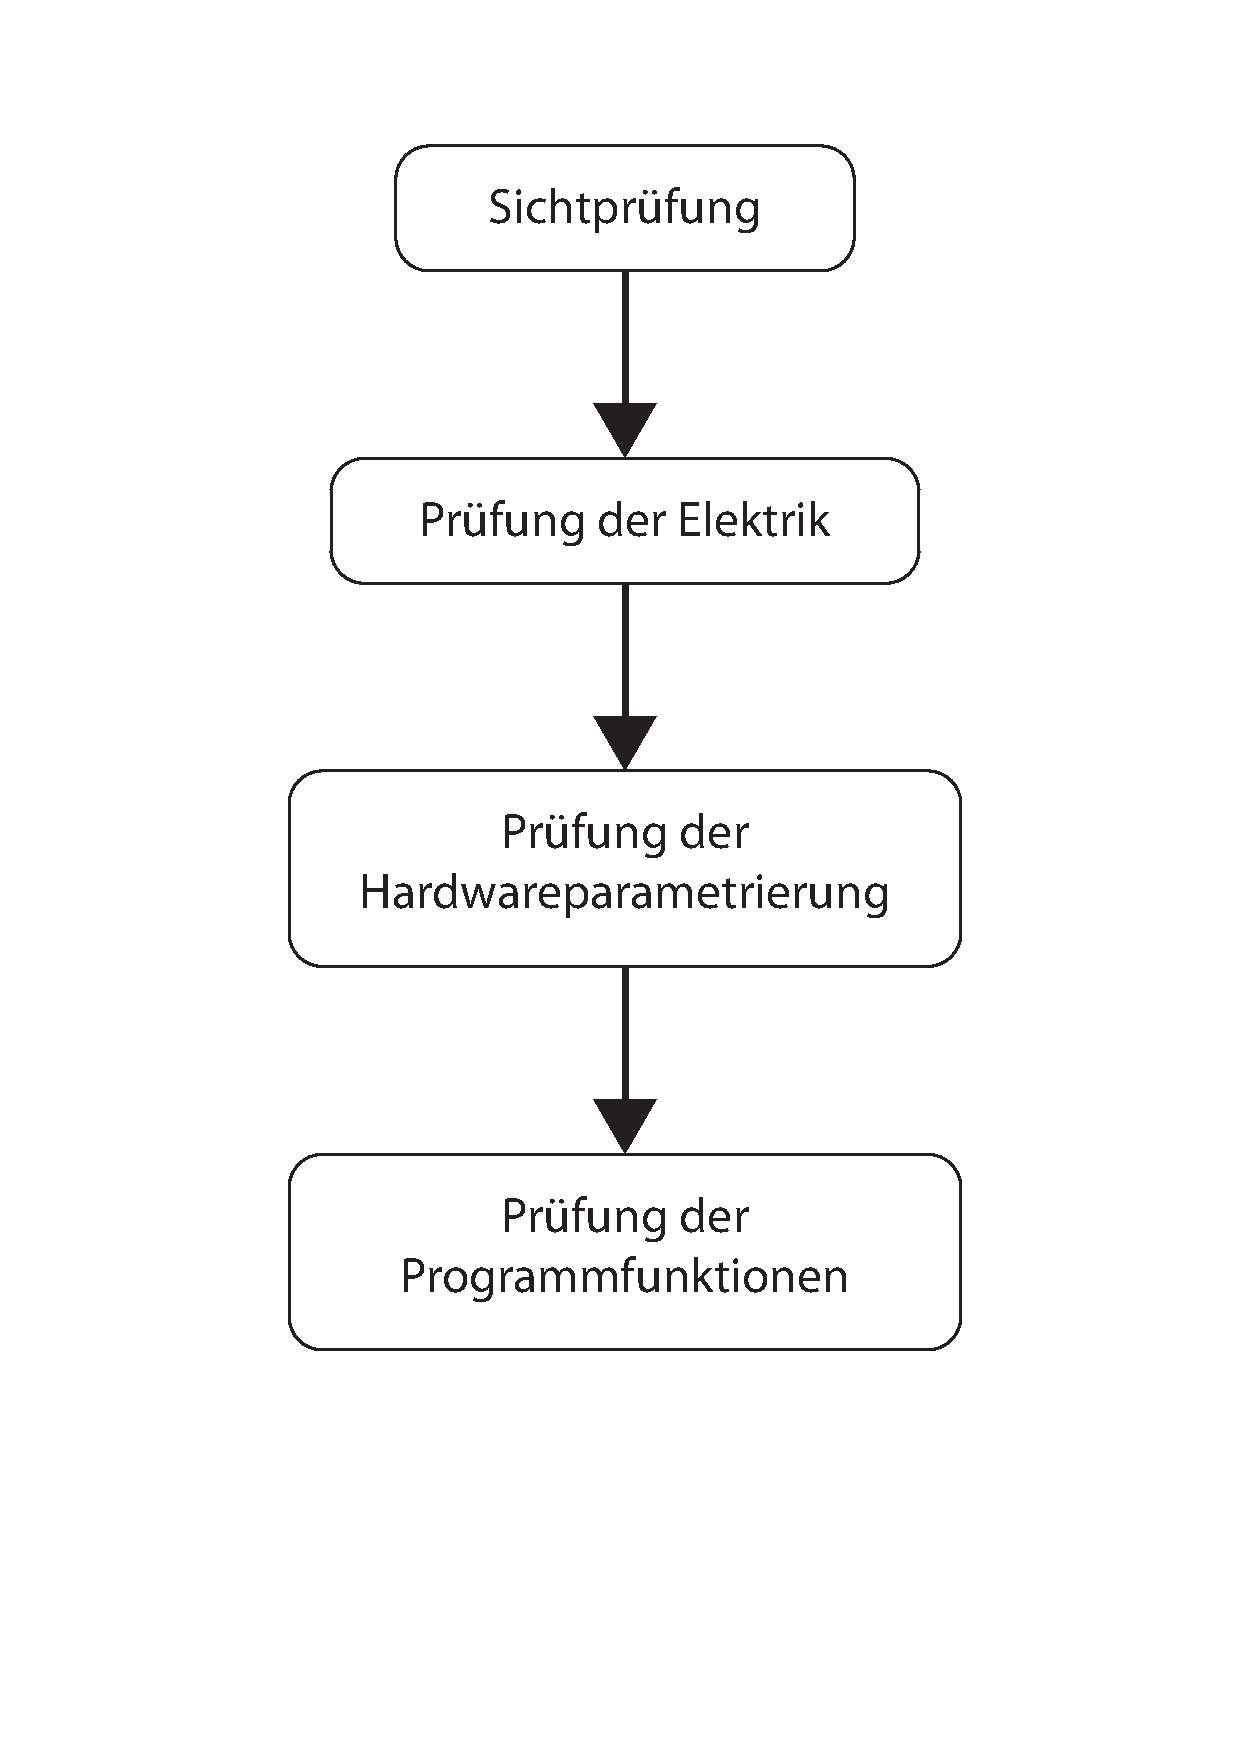
\includegraphics[width=0.5\textwidth]{Images/pruefablauf.pdf}
    \caption[Prüfablauf]{Ablauf zur schrittweisen Verifizierung der Testspezifikationen}
    \label{fig:my-img50}
\end{figure}

Die Protokollierung der Tests erfolgt nach der vorgenommenen Einteilung des dargestellten Diagrammes. Die einzelnen Punkte werden in den nachfolgenden Unterabschnitten abgearbeitet. Erneut kommt eine tabellarische Darstellung zum Einsatz, in der einzelne Testfälle mit den Schlüsselwörtern \textbf{bestanden}, \textbf{nicht bestanden} und \textbf{nicht getestet} protokolliert werden. Nicht durchgeführte Tests müssen nachgeholt werden. Ist ein Testfall nicht bestanden, so wird im anschließenden Unterkapitel die Korrektur der Implementierung diskutiert.

\subsubsection{Sichtprüfung}
% Vorhandensein Endlagen, Not-Halt-Taster, Lichtvorhang, Bedienelemente, Signalsäule
Die Sichtprüfung stellt den ersten Schritt in der Verifizierung der Testspezifikationen dar. Ziel ist es die Laboranlage durch eine visuelle Inspektion auf das Vorhandensein von allen geforderten Hardwarekomponenten zu untersuchen. Der durchgeführte Test bezieht sich dabei auf den Testfall \textit{TF\_01} (siehe \autoref{tab:my-table60}). Die protokollierten Ergebnisse sind in der nachfolgenden Tabelle aufgeführt.

\begin{longtable}[C]{| R{0.1\linewidth} | R{0.62\linewidth} | R{0.2\linewidth} | }
    \hline
    \textbf{Nr.}    &   \textbf{Testfall}                                                       &   \textbf{Ergebnis}   \\ \hline
    1               &   Steuerung \acs{lmc} 400c wurde verbaut                                  &   bestanden           \\ \hline
    2               &   Netzteil \acs{lxm} 62P wurde verbaut                                    &   bestanden           \\ \hline
    3               &   Servoregler \acs{lxm} 62D wurde verbaut                                 &   bestanden           \\ \hline
    4               &   Steuerung Wago PFC200 wurde verbaut                                     &   bestanden           \\ \hline
    5               &   Sicherheitssteuerung \acs{slc} 100 wurde verbaut                        &   bestanden           \\ \hline
    6               &   Modicon TM5 digitales Eingangsmodul wurde verbaut                       &   bestanden           \\ \hline
    7               &   Modicon TM5 digitales Ausgangsmodul wurde verbaut                       &   bestanden           \\ \hline
    8               &   Modicon TM5 analoges Eingangsmodul wurde verbaut                        &   bestanden           \\ \hline
    9               &   Modicon TM5 analoges Ausgangsmodul wurde verbaut                        &   bestanden           \\ \hline
    10              &   Modicon TM5 SERCOS III Bus-Interface wurde verbaut                      &   bestanden           \\ \hline
    11              &   Wago Leistungsklemme wurde verbaut                                      &   bestanden           \\ \hline
    12              &   Ethernetswitch wurde verbaut                                            &   bestanden           \\ \hline
    13              &   Vier Endlagesensoren wurden verbaut                                     &   bestanden           \\ \hline
    14              &   Zwei Not-Halt Taster wurden verbaut                                     &   bestanden           \\ \hline
    15              &   XUS Lichtvorhang wurde verbaut                                          &   bestanden           \\ \hline
    16              &   Ampel (rot/grün) wurde verbaut                                          &   bestanden           \\ \hline
    17              &   Schaltschrank an Gehäuse montiert                                       &   bestanden           \\ \hline
    18              &   Schaltschrankforderseite besitzt geforderte Bedienelemente              &   bestanden           \\ \hline
    19              &   Seiten des Gehäuses sind mit Plexiglasscheiben                          &   nicht bestanden     \\ \hline
    20              &   Kabel an den beweglichen Achsen sind in E-Ketten verlegt                &   bestanden           \\ \hline
    21              &   Die Laboranlage besitzt zwei bewegliche Achsen (x/z)                    &   bestanden           \\ \hline
    22              &   An jeder Achse ist ein Servomotor verbaut                               &   bestanden           \\ \hline
    23              &   Die z-Achse besitzt einen Greifarm                                      &   nicht bestanden     \\ \hline
    24              &   Am Greifarm ist ein Greifer montiert                                    &   nicht bestanden     \\ \hline
    25              &   24 \si{V}-Ebene ist über einen Leitungsschutzschalter abgesichert       &   bestanden           \\ \hline
    26              &   400 \si{V}-Ebene ist über einen Leitungsschutzschalter abgesichert      &   bestanden           \\ \hline
    27              &   Es wurde ein Netzschütz verbaut                                         &   nicht bestanden     \\ \hline
    28              &   Es wurde eine Netzdrossel verbaut                                       &   nicht bestanden     \\ \hline
    \caption[Sichtprüfung]{Testprotokoll - Sichtprüfung des mehrachsigen Positioniersystems}
    \label{tab:my-table90}
\end{longtable}

\subsubsection{Prüfung der Elektrik}
% Können die Betriebsmittel eingeschalten werden, ist alles richtig verdrahtet?
Nach Abschließen der Sichtprüfung des Systems kann mit der Prüfung der Elektronik fortgesetzt werden. Konkret soll über die nachfolgende Testung sichergestellt werden, dass alle Steuerungskomponenten sowie Sensoren und Aktuatoren richtig verdrahtet sind und eingesetzt werden können. Dazu wird der Testfall \textit{TF\_02} herangezogen (siehe \autoref{tab:my-table61}). Die durch die Nichterfüllung des ersten Testfalls betroffenen Testkriterien werden im Feld \textit{Ergebnis} frei gelassen.

\begin{longtable}[C]{| R{0.1\linewidth} | R{0.62\linewidth} | R{0.2\linewidth} | }
    \hline
    \textbf{Nr.}    &   \textbf{Testfall}                                                               &   \textbf{Ergebnis}   \\ \hline
    1               &   \acs{lmc}400c fährt nach Einschalten des Systems über den Hauptschalter hoch    &   bestanden           \\ \hline
    2               &   Wago PFC200 fährt nach Einschalten des Systems über den Hauptschalter hoch      &   bestanden           \\ \hline
    3               &   Status-LED des Netzteils \acs{lxm} 62P aktiv                                    &   bestanden           \\ \hline
    4               &   Power-LED des Netzteils \acs{lxm} 62P aktiv                                     &   bestanden           \\ \hline
    5               &   Status-LED des Servoreglers \acs{lxm} 62D aktiv                                 &   bestanden           \\ \hline
    6               &   Power-LED des \acs{slc}100 aktiv                                                &   bestanden           \\ \hline
    7               &   Power-LED des Modicon TM5 Bus Interface aktiv                                   &   bestanden           \\ \hline
    8               &   LEDs der Modicon TM5 \acs{ea}-Module aktiv                                      &   bestanden           \\ \hline
    9               &   Ready-Relais-Output des Netzteils mit Netzschütz verdrahtet                     &   ---                 \\ \hline
    10              &   Netzschütz schaltet 400 \si{V} Spannungsversorgung des Netzteils                &   ---                 \\ \hline
    11              &   Initiatorklemmen der Endlagesensoren leuchten im nicht geschalteten Zustand     &   bestanden           \\ \hline
    12              &   Initiatorklemmen des Lichtvorhangs leuchten im nicht ausgelösten Zustand        &   bestanden           \\ \hline
    13              &   LEDs der Not-Halt Sicherheitseingänge leuchten antivalent                       &   bestanden           \\ \hline
    14              &   Initiatorklemmen der Bedienelemente leuchten entsprechend des Schaltzustandes   &   nicht bestanden     \\ \hline
    15              &   Leitungsschutzschalter für 400 \si{V}-Ebene kann diese schalten                 &   bestanden           \\ \hline
    16              &   Leitungsschutzschalter für 24 \si{V}-Ebene kann diese schalten                  &   bestanden           \\ \hline
    17              &   Iverter-Enable Eingang des Servoreglers \acs{lxm} 62D ist mit dem ersten Sicherheitsausgang verdrahtet   &   bestanden           \\ \hline
    18              &   Netzdrossel ist in 400 \si{V}-Ebene verdrahtet                                  &   ---                 \\ \hline
    \caption[Prüfung der Elektrik]{Testprotokoll - Prüfung der Verdrahtung des Systems}
    \label{tab:my-table91}
\end{longtable}

\subsubsection{Prüfung der Geräteparametrierung}
% läuft der sercos, können daten zwischen den PLCs versendet werden, ist der Servoregler eingerichtet, ist das Netzteil eingerichtet, funktionieren die sicheren Ein-/Ausgänge, könne Daten per OPC ausgelesen werden?
Bevor konkrete Funktionen verifiziert werden können, müssen zunächst die eingestellten Geräteparameter geprüft werden. Dabei wird Bezug genommen auf den Testfall \textit{TF\_03} (Siehe \autoref{tab:my-table62}). Die Nichterfüllung voraussetzender Testkriterien führt auch in dieser Tabelle zu der Freilassung des Ergebnisfeldes. Die Überprüfung und Verifizierung der Geräteparameter erfolgt in der Software \textit{MachineExpert LogicBuilder}. Sämtliche zu treffende Einstellungen sind Voraussetzung für die korrekte Inbetriebnahme. Ist ein Testkriterium nicht erfüllt, da eine Systemkomponente nicht vorhanden ist oder Änderungen am Aufbau der Anlage vorgenommen wurden, muss die Parametrierung angepasst werden, sodass der Testfall zu 100\% bestanden wird. Ein Nichtbestehen sorgt zu einer Fehlermeldung im Programm oder verhindert die Ausführung von Systemfunktionen.

\begin{longtable}[C]{| R{0.1\linewidth} | R{0.62\linewidth} | R{0.2\linewidth} | }
    \hline
    \textbf{Nr.}    &   \textbf{Testfall}                                                                                                           &   \textbf{Ergebnis}   \\ \hline
    1               &   Steuerung \acs{lmc}400c des Positioniersystems wurde in Steuerungsauswahl selektiert                                        &   bestanden           \\ \hline
    2               &   Jeder SERCOS III Busteilnehmer besitz eine eigene topologische Adresse entsprechend der realen Verdrahtungsreihenfolge      &   bestanden           \\ \hline
    3               &   Der SERCOS III Bus befindet sich in Phase 4 (Ringkommunikations) und ermöglicht Datentransfer zwischen allen Busteilnehmern &   bestanden           \\ \hline
    4               &   Physikalische Parameter der Achsen wurden in den Servoreglereinstallungen aufgenommen                                       &   bestanden           \\ \hline
    5               &   Das Netzteil ist auf 400 \si{V} und 3-phasige Überwachung eingestellt (\textit{PhaseCheckMode}, \textit{MainsVoltageMode})  &   bestanden           \\ \hline
    6               &   Diagnosemaske für offene Ausgänge des \acs{lmc} wurde gesetzt (\textit{OpenDiagMask})                                       &   bestanden           \\ \hline
    7               &   Adressbereiche des \acs{slc} wurden für den Datenaustausch mit dem \acs{lmc} freigegeben (\textit{LMC2SLCNumberOfBOOLs})   &   bestanden           \\ \hline
    8               &   \acs{ea}-Abbild wurde in einer globalen Variablenliste angelegt                                                             &   bestanden           \\ \hline
    9               &   Sichere \acs{ea}-Module wurden entsprechend der zeitlichen Anforderungen parametriert                                       &   bestanden           \\ \hline
    \caption[Prüfung der Geräteparametrierung]{Testprotokoll - Prüfung der Geräteparametrierung in der Steuerungskonfiguration}
    \label{tab:my-table92}
\end{longtable}

\subsubsection{Prüfung der Programmfunktionen}
% Führt die Programmierung des Systems zum geplanten Verhalten?
Zuletzt werden die eigentlichen Funktionen des mehrachsigen Positioniersystems verifiziert. Anders als die bisherigen Tabellen im Testprotokoll sind nun nicht mehrere Testkriterien in einer Tabelle aufgeführt. Jeder Testfall eine Funktion betreffend besitzt eine eigene Tabelle mit allen geforderten Kriterien für die Erfüllung des jeweiligen Testfalls. Die nachfolgenden Tabellen beziehen sich auf die Testfälle \textit{TF\_04} bis \textit{TF\_12}. Der betrachtete Testfall wird im Titel der jeweiligen Tabelle referenziert.

\begin{longtable}[C]{| R{0.1\linewidth} | R{0.62\linewidth} | R{0.2\linewidth} | }
    \hline
    \textbf{Nr.}    &   \textbf{Testfall}                                                                                                           &   \textbf{Ergebnis}   \\ \hline
    1               &   Weiße Taster leuchten nach Handmodusauswahl                                                                                 &   nicht bestanden     \\ \hline
    2               &   Handmodus-Button wird nach Handmodusauswahl in \acs{gui} grün hinterlegt                                                    &   bestanden           \\ \hline
    3               &   Bestätigung der Auswahl führt zur Aktivierung der grünen LED des Start-Tasters                                              &   nicht bestanden     \\ \hline
    4               &   Bestätigung der Auswahl führt zum Anlegen der Aufgabe in der \acs{gui}                                                      &   bestanden           \\ \hline
    5               &   Tasten des vierfach Drucktasters führt zu Bewegungen der jeweiligen Achse                                               &   nicht bestanden     \\ \hline
    6               &   Drücken der \textit{Jog+} und \textit{Jog-} Buttons führt nach Auswahl der Achse zu Bewegungen an dieser Achse              &   bestanden           \\ \hline
    7               &   Tasten der weißen Bedienelemente bewegt den Greifer \bzw den Greifarm                                                       &   nicht bestanden     \\ \hline
    \caption[Prüfung Handmodus]{Testprotokoll - Prüfung der Handmodusfunktionalität siehe \autoref{tab:my-table63}}
    \label{tab:my-table93}
\end{longtable}

\begin{longtable}[C]{| R{0.1\linewidth} | R{0.62\linewidth} | R{0.2\linewidth} | }
    \hline
    \textbf{Nr.}    &   \textbf{Testfall}                                                                                                           &   \textbf{Ergebnis}   \\ \hline
    1               &   Positioniersystem arbeitet Absolut-Positionieraufgaben nach Programmvorgaben ohne Nutzereingaben ab                         &   nicht getestet      \\ \hline
    2               &   Positioniersystem fährt programmatisch vorgegebene Trajektorien ohne Nutzereingaben ab                                      &   nicht getestet      \\ \hline
    3               &   System führt automatische Greifoperationen zur Aufnahme und Ablage von Transportobjekten durch                              &   ---                 \\ \hline
    4               &   System fährt leer nach Betätigung des Stop-Tasters                                                                          &   nicht getestet      \\ \hline
    \caption[Prüfung Automatikmodus]{Testprotokoll - Prüfung des Automatikmodus siehe \autoref{tab:my-table64}}
    \label{tab:my-table94}
\end{longtable}

\begin{longtable}[C]{| R{0.1\linewidth} | R{0.62\linewidth} | R{0.2\linewidth} | }
    \hline
    \textbf{Nr.}    &   \textbf{Testfall}                                                                                                           &   \textbf{Ergebnis}   \\ \hline
    1               &   x-Achse bewegt sich langsam bei niedrigster Geschwindigkeitseinstellung am oberen \acs{poti}                                &   ---                 \\ \hline
    2               &   z-Achse bewegt sich langsam bei niedrigster Geschwindigkeitseinstellung am unteren \acs{poti}                               &   ---                 \\ \hline
    3               &   x-Achse bewegt sich schnell bei höchster Geschwindigkeitseinstellung am oberen \acs{poti}                                   &   ---                 \\ \hline
    4               &   z-Achse bewegt sich schnell bei höchster Geschwindigkeitseinstellung am unteren \acs{poti}                                  &   ---                 \\ \hline
    \caption[Prüfung Geschwindigkeitsvorgabe]{Testprotokoll - Prüfung der Geschwindigkeitsvorgabe siehe \autoref{tab:my-table65}}
    \label{tab:my-table95}
\end{longtable}

\begin{longtable}[C]{| R{0.1\linewidth} | R{0.62\linewidth} | R{0.2\linewidth} | }
    \hline
    \textbf{Nr.}    &   \textbf{Testfall}                                                                                                           &   \textbf{Ergebnis}   \\ \hline
    1               &   Erreichen der rechten Endlage stoppt/verhindert Bewegung der x-Achse nach rechts                                            &   bestanden           \\ \hline
    2               &   Erreichen der linken Endlage stoppt/verhindert Bewegung der x-Achse nach links                                              &   bestanden           \\ \hline
    3               &   Erreichen der oberen Endlage stoppt/verhindert Bewegung der z-Achse nach oben                                               &   bestanden           \\ \hline
    4               &   Erreichen der unteren Endlage stoppt/verhindert Bewegung der z-Achse nach unten                                             &   bestanden           \\ \hline
    5               &   Bewegungen in Endlagennähe sind gedämpft (verringerte Geschwindigkeit, Beschleunigung)                                      &   nicht bestanden     \\ \hline
    \caption[Prüfung Endlagenfunktionalität]{Testprotokoll - Prüfung der Endlagenfunktionalität siehe \autoref{tab:my-table66}}
    \label{tab:my-table96}
\end{longtable}

\begin{longtable}[C]{| R{0.1\linewidth} | R{0.62\linewidth} | R{0.2\linewidth} | }
    \hline
    \textbf{Nr.}    &   \textbf{Testfall}                                                                                                           &   \textbf{Ergebnis}   \\ \hline
    1               &   Erster sicherer Eingang detektiert Lichtvorhangauslösung nach spätestens 50\si{ms}                                          &   bestanden           \\ \hline
    2               &   Zweiter sicherer Eingang detektiert Lichtvorhangauslösung nach spätestens 50\si{ms}                                         &   bestanden           \\ \hline
    3               &   Not-Halt-Auslösung stoppt jegliche Bewegung nach spätestens 200\si{ms}                                                      &   nicht getestet      \\ \hline
    4               &   Not-Halt-Auslösung schaltet Servoregler nach spätestens 250\si{ms} ab                                                       &   bestanden           \\ \hline
    5               &   Der zurückgelegte Weg einer Achse nach Not-Halt Auslösung ist kleiner als 5\si{cm}                                          &   bestanden           \\ \hline
    \caption[Prüfung funktionale Sicherheit]{Testprotokoll - Prüfung der funktionalen Sicherheit siehe \autoref{tab:my-table67}}
    \label{tab:my-table97}
\end{longtable}

\begin{longtable}[C]{| R{0.1\linewidth} | R{0.62\linewidth} | R{0.2\linewidth} | }
    \hline
    \textbf{Nr.}    &   \textbf{Testfall}                                                                                                           &   \textbf{Ergebnis}   \\ \hline
    1               &   Bewegungsbefehle führen nach Not-Halt Auslösung zu keiner Bewegung                                                          &   bestanden           \\ \hline
    2               &   Betätigung des Reset-Tasters ermöglicht die erneute Ausführung von Bewegungsbefehlen                                        &   ---                 \\ \hline
    3               &   Quittieren des Fehlers aus der \acs{gui} ermöglicht die erneute Ausführung von Bewegungsbefehlen                            &   bestanden           \\ \hline
    \caption[Prüfung Reset-Funktion]{Testprotokoll - Prüfung der Reset-Funktion siehe \autoref{tab:my-table68}}
    \label{tab:my-table98}
\end{longtable}

\begin{longtable}[C]{| R{0.1\linewidth} | R{0.62\linewidth} | R{0.2\linewidth} | }
    \hline
    \textbf{Nr.}    &   \textbf{Testfall}                                                                                                                   &   \textbf{Ergebnis}   \\ \hline
    1               &   Software \textit{MachineExpert LogicBuilder} auf jedem Laborrechner installiert                                                     &   bestanden           \\ \hline
    2               &   Steuerung \acs{lmc}400c des Positioniersystems kann bei Steuerungsauswahl von jedem Laborcomputer gefunden werden                   &   bestanden           \\ \hline
    3               &   Betätigung des Buttons \glqq visuelles Signalisieren\grqq{} in Steuerungsauswahloberfläche lässt Status-LED am \acs{lmc} blinken    &   bestanden           \\ \hline
    4               &   Es können Programme von jedem Rechner im Labor auf die Steuerung gespielt werden                                                    &   bestanden           \\ \hline
    5               &   Jeder Laborcomputer kann sich auf der Steuerung einloggen                                                                           &   bestanden           \\ \hline
    \caption[Prüfung Programmierschnittstelle]{Testprotokoll - Prüfung der Programmierschnittstelle \autoref{tab:my-table69}}
    \label{tab:my-table99}
\end{longtable}

\begin{longtable}[C]{| R{0.1\linewidth} | R{0.62\linewidth} | R{0.2\linewidth} | }
    \hline
    \textbf{Nr.}    &   \textbf{Testfall}                                                                                                           &   \textbf{Ergebnis}   \\ \hline
    1               &   OPC Server auf \acs{lmc} kann über die Software \textit{OPC-Watch} gefunden werden                                          &   bestanden           \\ \hline
    2               &   OPC Server auf PFC200 kann über die Software \textit{OPC-Watch} gefunden werden                                             &   nicht getestet      \\ \hline
    3               &   Es können Daten vom \acs{lmc} über den OPC Client der \textit{OPC-Watch} Software ausgelesen werden                         &   bestanden           \\ \hline
    4               &   Es können Daten vom PFC200 über den OPC Client der \textit{OPC-Watch} Software ausgelesen werden                            &   nicht getestet      \\ \hline
    5               &   Es können Daten aus dem OPC Client angepasst und zurück an den \acs{lmc} übertragen werden                                  &   bestanden           \\ \hline
    6               &   Es können Daten aus dem OPC Client angepasst und zurück an den PFC200 übertragen werden                                     &   nicht getestet      \\ \hline
    \caption[Prüfung OPC Kommunikation]{Testprotokoll - Prüfung der OPC UA Schnittstelle \autoref{tab:my-table80}}
    \label{tab:my-table100}
\end{longtable}

\newpage

\begin{longtable}[C]{| R{0.1\linewidth} | R{0.62\linewidth} | R{0.2\linewidth} | }
    \hline
    \textbf{Nr.}    &   \textbf{Testfall}                                                                                                           &   \textbf{Ergebnis}   \\ \hline
    1               &   Ampel leuchtet dauerhaft grün, wenn das System im Leerlauf ist (keine Bewegungen der Achsen)                                &   bestanden           \\ \hline
    2               &   Ampel leuchtet dauerhaft rot, wenn das System im Fehlerzustand ist (Not-Halt ausgelöst)                                     &   bestanden           \\ \hline
    3               &   Ampel blinkt abwechselnd rot und grün, wenn das System Achsbewegungen durchführt                                            &   bestanden           \\ \hline
    \caption[Prüfung Signalampel]{Testprotokoll - Prüfung der Signalampel \autoref{tab:my-table81}}
    \label{tab:my-table101}
\end{longtable}

\end{document}